\documentclass[11pt]{article}

\usepackage[margin=1in]{geometry}
\usepackage{microtype}

\usepackage{amsmath}
\usepackage{amssymb}
\usepackage{amsthm}
\usepackage{mathtools}

\usepackage{graphicx}
\graphicspath{{figures/}}
\usepackage{booktabs}
\usepackage{array}
\usepackage{tabularx}
\usepackage{siunitx}
\usepackage[font=small,labelfont=bf]{caption}
\usepackage[section]{placeins}

\usepackage{xr-hyper}
\usepackage{hyperref}
\usepackage[nameinlink,capitalise,noabbrev]{cleveref}

\usepackage[numbers,sort&compress]{natbib}

% References to the paper resolve through main.aux; build main.tex first.
\externaldocument{main}

% Common macros and theorem environments for the arXiv manuscript.

% \Pr is defined by amsmath (as an operator), so use \PP for probability.
\newcommand{\PP}{\mathbb{P}}
\newcommand{\ind}{\mathbf{1}}
\newcommand{\countfrac}[2]{\makebox[1.35em][r]{#1}/\makebox[1.35em][l]{#2}}
\newcommand{\winloss}[2]{\makebox[1.35em][r]{#1}--\makebox[1.0em][l]{#2}}
\newcommand{\tablehead}[1]{\multicolumn{1}{c}{#1}}
\newcolumntype{L}[1]{>{\raggedright\arraybackslash}p{#1}}
\newcolumntype{C}[1]{>{\centering\arraybackslash}p{#1}}
\newcolumntype{Y}{>{\raggedright\arraybackslash}X}
\sisetup{
  group-separator={,},
  group-minimum-digits=4,
  input-ignore={,},
  retain-explicit-plus,
  table-number-alignment=center,
  table-text-alignment=center
}

\DeclareMathOperator*{\argmin}{arg\,min}

\theoremstyle{plain}
\newtheorem{theorem}{Theorem}
\newtheorem{lemma}{Lemma}
\newtheorem{corollary}{Corollary}
\newtheorem{proposition}{Proposition}
\AddToHook{env/theorem/begin}{\crefalias{section}{theorem}}
\AddToHook{env/lemma/begin}{\crefalias{section}{lemma}}
\AddToHook{env/corollary/begin}{\crefalias{section}{corollary}}

\theoremstyle{definition}
\newtheorem{definition}{Definition}
\AddToHook{env/definition/begin}{\crefalias{section}{definition}}

\theoremstyle{remark}
\newtheorem{remark}{Remark}
\AddToHook{env/remark/begin}{\crefalias{section}{remark}}

\hypersetup{
  hidelinks,
  pdftitle={Supplement to Conditional Inference Trees and Forests for Feature Selection},
  pdfauthor={Robert Milletich, Justin Downes, Steve Goley, Newel Hirst}
}

\renewcommand{\thesection}{S\arabic{section}}
\renewcommand{\thetable}{S\arabic{table}}
\renewcommand{\thefigure}{S\arabic{figure}}

\title{Supplement to ``Conditional Inference Trees and Forests for Feature Selection''}
\author{%
  Robert Milletich, Justin Downes, Steve Goley, Newel Hirst\\
  Amazon Web Services\\
  \texttt{\char`\{rmilleti,jusdow,sgoley,nhirst\char`\}@amazon.com}
}
\date{}

\begin{document}
\maketitle

This supplement holds the tables and figures behind statements in the paper
that the paper reports in its text. Section, table, and figure numbers without
the prefix S refer to the paper.

\section{Benchmark stability}
\label{app:benchmark-stability}

\Cref{tab:complete-case-pairwise-ci} supports the interval statements of
\cref{sec:experiments-real}. It gives the paired difference of CIF against
every other method on the complete-case panels, 16 contrasts in classification
and 17 in regression, with the percentile bootstrap intervals that
\cref{tab:conditional-inference-comparisons} reports for the conditional
inference comparisons. In classification the intervals favor CIF against CIT,
ctree, cforest, the single trees, the permutation filters, PI, and CPI; in
regression they exclude zero against the filters, PI, CPI, LightGBM, and ctree.
Every analysis in this section uses the configurations selected for the main
benchmark (\cref{sec:experiments-repro}).

\begin{table}[!htbp]
  \centering
  \footnotesize
  \setlength{\tabcolsep}{3.5pt}
  \renewcommand{\arraystretch}{0.95}
  \begin{tabular}{@{}l S[table-format=-1.3] c c @{\hspace{1.5em}} l S[table-format=-1.3] c c@{}}
    \toprule
    \multicolumn{4}{c}{Classification} & \multicolumn{4}{c}{Regression} \\
    \cmidrule(lr){1-4}\cmidrule(l){5-8}
    \tablehead{Compared with} & {Mean} & 95\% interval & Wins--losses &
    \tablehead{Compared with} & {Mean} & 95\% interval & Wins--losses \\
    \midrule
    RF-RFE & -0.027 & [$-$0.038, $-$0.016] & \winloss{1}{12} & ExtraTrees & -0.039 & [$-$0.124, 0.042] & \winloss{2}{4} \\
    XGBoost & -0.012 & [$-$0.022, $-$0.004] & \winloss{4}{9} & CatBoost & 0.024 & [$-$0.001, 0.049] & \winloss{4}{2} \\
    RF & -0.004 & [$-$0.013, 0.006] & \winloss{5}{8} & RF-RFE & -0.080 & [$-$0.181, 0.019] & \winloss{2}{4} \\
    LightGBM & -0.015 & [$-$0.024, $-$0.006] & \winloss{3}{10} & RF & -0.007 & [$-$0.043, 0.023] & \winloss{3}{3} \\
    Boruta & 0.007 & [$-$0.014, 0.031] & \winloss{7}{6} & RT & -0.013 & [$-$0.054, 0.030] & \winloss{3}{3} \\
    CatBoost & -0.003 & [$-$0.015, 0.010] & \winloss{5}{8} & cforest & 0.027 & [$-$0.032, 0.090] & \winloss{5}{1} \\
    ExtraTrees & 0.006 & [$-$0.007, 0.020] & \winloss{7}{6} & DT & 0.129 & [$-$0.001, 0.304] & \winloss{3}{3} \\
    cforest & 0.013 & [0.002, 0.024] & \winloss{9}{4} & Boruta & 0.135 & [$-$0.006, 0.368] & \winloss{3}{3} \\
    DT & 0.035 & [0.012, 0.060] & \winloss{12}{1} & PC filter & 0.154 & [0.028, 0.333] & \winloss{5}{1} \\
    RDC filter & 0.034 & [0.016, 0.053] & \winloss{10}{3} & LightGBM & 0.467 & [0.003, 1.227] & \winloss{4}{2} \\
    PI & 0.122 & [0.079, 0.170] & \winloss{13}{0} & XGBoost & 0.066 & [$-$0.012, 0.164] & \winloss{4}{2} \\
    MC filter & 0.062 & [0.027, 0.102] & \winloss{12}{1} & RDC filter & 0.335 & [0.032, 0.814] & \winloss{5}{1} \\
    RT & 0.061 & [0.038, 0.086] & \winloss{13}{0} & CIT & 0.308 & [$-$0.002, 0.766] & \winloss{5}{1} \\
    ctree & 0.049 & [0.026, 0.073] & \winloss{11}{2} & ctree & 0.202 & [0.029, 0.421] & \winloss{4}{2} \\
    CIT & 0.044 & [0.027, 0.062] & \winloss{13}{0} & PI & 0.277 & [0.018, 0.731] & \winloss{4}{2} \\
    CPI & 0.198 & [0.135, 0.262] & \winloss{13}{0} & DC filter & 0.262 & [0.031, 0.543] & \winloss{5}{1} \\
    \multicolumn{4}{c}{} & CPI & 0.808 & [0.035, 2.197] & \winloss{5}{1} \\
    \bottomrule
  \end{tabular}
  \caption{Paired differences of CIF against every other method on the
  complete-case panels, 13 classification and 6 regression datasets. Mean is
  the mean over datasets of CIF minus the compared method in dataset-mean
  score, balanced accuracy in classification and $R^2$ in regression, averaged
  over downstream learners and standard values of $k$. The 95\% interval is a
  percentile bootstrap interval over the dataset-level differences from
  20{,}000 replicates with a fixed seed; the intervals are unadjusted post-hoc
  contrasts. Wins and losses count datasets; no exact ties occurred. Rows follow
  the order of \cref{tab:method-main-comparison}.}
  \label{tab:complete-case-pairwise-ci}
\end{table}

\subsection{Benchmark exclusions}

\Cref{tab:coverage-skips} lists, by dataset and method, the 34 classification
runs excluded from the benchmark, whose counts \cref{app:methods} summarizes.

\begin{table}[!htbp]
  \centering
  \footnotesize
  \setlength{\tabcolsep}{4pt}
  \begin{tabular}{@{}llccl@{}}
    \toprule
    \tablehead{Dataset} & \tablehead{Method} & {Configurations} & {Seed runs} & \tablehead{Basis} \\
    \midrule
    \nolinkurl{gisette} & CIT with the RDC selector & 2 & 8 & host fault \\
    \nolinkurl{gisette} & ctree & 1 & 5 & incomplete \\
    \nolinkurl{isolet} & CIF with the RDC selector & 2 & 4 & host fault \\
    \nolinkurl{isolet} & CIT with the RDC selector & 2 & 6 & host fault \\
    \nolinkurl{isolet} & cforest & 1 & 5 & incomplete \\
    \nolinkurl{isolet} & ctree & 1 & 5 & incomplete \\
    \nolinkurl{orlraws10P} & CIT with the RDC selector & 1 & 1 & author directed \\
    \bottomrule
  \end{tabular}
  \caption{Classification benchmark exclusions. Each seed run is one method
  configuration on one dataset with one seed; 34 runs are excluded in total,
  and all are operational exclusions. Incomplete rows are partykit ctree and
  cforest runs that did not complete; the 18 host-fault runs are RDC-selector
  CIT and CIF runs lost to a host fault; the
  single \nolinkurl{orlraws10P} run was excluded by author decision. No regression runs
  are excluded.}
  \label{tab:coverage-skips}
\end{table}

\subsection{LODO configuration sensitivity}

These tables support the leave-one-dataset-out (LODO) positions of CIF in
\cref{sec:experiments-real}. Each LODO run selects configurations on all but
one dataset of the panel, scores the held-out dataset, and averages scores and
ranks over downstream learners and standard values of $k$.
\Cref{tab:lodo-config-sensitivity,tab:lodo-config-sensitivity-allmethod} report
the complete-case and all-method panels. Every single-configuration family
keeps its held-out score exactly, as it must, since reselection changes only
the tuned families. Its mean rank moves only as the tuned families are
reselected around it, by at most 0.05 in classification and 0.125 in
regression. On the all-method panels CIF loses 0.002 balanced accuracy and
0.008 $R^2$ under reselection, and XGBoost loses 0.03 $R^2$ (0.270 against
0.241). The one large reselection effect is cforest in regression, whose
alternative configuration is chosen on one holdout and scores far lower there
(mean $R^2$ 0.30 against 0.20).

\begin{table}[!htbp]
  \centering
  \fontsize{8}{9.1}\selectfont
  \setlength{\tabcolsep}{2.5pt}
  \renewcommand{\arraystretch}{1.0}
  \begin{tabular*}{\linewidth}{@{\extracolsep{\fill}}l
    S[table-format=2.2]
    S[table-format=2.2]
    S[table-format=1.3]
    S[table-format=1.0]
    c
    @{\hspace{0.8em}}
    l
    S[table-format=2.2]
    S[table-format=2.2]
    S[table-format=-1.3]
    S[table-format=1.0]
    c@{}}
    \toprule
    \multicolumn{6}{c}{Classification} &
    \multicolumn{6}{c}{Regression} \\
    \cmidrule(lr){1-6}\cmidrule(l){7-12}
    \tablehead{Method} & {LODO} & {Fixed} & {Score} & {Settings} & {Main} &
    \tablehead{Method} & {LODO} & {Fixed} & {Score} & {Settings} & {Main} \\
    \midrule
    RF-RFE & 2.54 & 2.54 & 0.825 & 1 & \countfrac{13}{13} & ExtraTrees & 4.67 & 4.67 & 0.292 & 1 & \countfrac{6}{6} \\
    LightGBM & 4.31 & 4.46 & 0.813 & 1 & \countfrac{13}{13} & CatBoost & 6.17 & 6.33 & 0.229 & 1 & \countfrac{6}{6} \\
    RF & 5.08 & 5.23 & 0.802 & 1 & \countfrac{13}{13} & RF-RFE & 6.67 & 6.67 & 0.333 & 1 & \countfrac{6}{6} \\
    CatBoost & 5.54 & 5.69 & 0.801 & 1 & \countfrac{13}{13} & RF & 6.83 & 7.00 & 0.260 & 1 & \countfrac{6}{6} \\
    XGBoost & 5.69 & 4.92 & 0.808 & 2 & \countfrac{11}{13} & RT & 7.00 & 7.00 & 0.266 & 1 & \countfrac{6}{6} \\
    Boruta & 6.23 & 6.38 & 0.791 & 1 & \countfrac{13}{13} & CIF & 7.33 & 7.00 & 0.240 & 2 & \countfrac{4}{6} \\
    ExtraTrees & 6.62 & 6.77 & 0.792 & 1 & \countfrac{13}{13} & XGBoost & 8.50 & 8.67 & 0.149 & 2 & \countfrac{5}{6} \\
    CIF & 6.85 & 6.38 & 0.793 & 2 & \countfrac{11}{13} & DT & 8.67 & 8.83 & 0.124 & 1 & \countfrac{6}{6} \\
    cforest & 8.23 & 8.46 & 0.785 & 1 & \countfrac{13}{13} & Boruta & 9.17 & 9.33 & 0.118 & 1 & \countfrac{6}{6} \\
    DT & 9.38 & 9.46 & 0.763 & 1 & \countfrac{13}{13} & LightGBM & 10.50 & 10.50 & -0.214 & 1 & \countfrac{6}{6} \\
    RDC filter & 10.69 & 10.85 & 0.764 & 1 & \countfrac{13}{13} & CIT & 10.67 & 10.50 & -0.206 & 2 & \countfrac{5}{6} \\
    ctree & 11.77 & 11.77 & 0.749 & 1 & \countfrac{13}{13} & cforest & 10.67 & 9.67 & 0.092 & 2 & \countfrac{5}{6} \\
    CIT & 12.15 & 12.15 & 0.754 & 1 & \countfrac{13}{13} & PI & 11.00 & 11.00 & -0.024 & 1 & \countfrac{6}{6} \\
    MC filter & 12.69 & 12.69 & 0.737 & 1 & \countfrac{13}{13} & ctree & 11.33 & 11.50 & 0.051 & 1 & \countfrac{6}{6} \\
    RT & 13.00 & 13.00 & 0.737 & 1 & \countfrac{13}{13} & PC filter & 11.67 & 11.83 & 0.099 & 1 & \countfrac{6}{6} \\
    PI & 15.73 & 15.73 & 0.676 & 1 & \countfrac{13}{13} & RDC filter & 12.50 & 12.67 & -0.082 & 1 & \countfrac{6}{6} \\
    CPI & 16.50 & 16.50 & 0.600 & 1 & \countfrac{13}{13} & DC filter & 13.50 & 13.67 & -0.009 & 1 & \countfrac{6}{6} \\
    \multicolumn{6}{c}{} & CPI & 14.17 & 14.17 & -0.554 & 1 & \countfrac{6}{6} \\
    \bottomrule
  \end{tabular*}
  \caption{LODO configuration sensitivity on the complete-case panels (13
  classification and 6 regression datasets). LODO is the mean rank when each
  held-out dataset is scored with configurations selected on the other
  datasets; Fixed is the mean rank on the same panel under the configuration
  selected on the full benchmark. Lower rank is better; rows are ordered by LODO
  rank within each task. Score is the mean held-out metric under LODO
  selection. Settings reports the number of distinct selected configurations;
  Main reports how often the main benchmark configuration is reselected. Ranks
  are computed within held-out datasets before averaging, so score order need
  not match rank order. Entries are mean ranks over the panel datasets; the difference between the fixed and LODO columns is the reported sensitivity.}
  \label{tab:lodo-config-sensitivity}
\end{table}

\begin{table}[!htbp]
  \centering
  \fontsize{8}{9.1}\selectfont
  \setlength{\tabcolsep}{2.5pt}
  \renewcommand{\arraystretch}{1.0}
  \begin{tabular*}{\linewidth}{@{\extracolsep{\fill}}l
    S[table-format=2.2]
    S[table-format=2.2]
    S[table-format=1.3]
    S[table-format=1.0]
    c
    @{\hspace{0.8em}}
    l
    S[table-format=2.2]
    S[table-format=2.2]
    S[table-format=-1.3]
    S[table-format=1.0]
    c@{}}
    \toprule
    \multicolumn{6}{c}{Classification} &
    \multicolumn{6}{c}{Regression} \\
    \cmidrule(lr){1-6}\cmidrule(l){7-12}
    \tablehead{Method} & {LODO} & {Fixed} & {Score} & {Settings} & {Main} &
    \tablehead{Method} & {LODO} & {Fixed} & {Score} & {Settings} & {Main} \\
    \midrule
    RF-RFE & 4.19 & 4.19 & 0.837 & 1 & \countfrac{21}{21} & ExtraTrees & 5.00 & 5.00 & 0.353 & 1 & \countfrac{8}{8} \\
    XGBoost & 5.81 & 5.81 & 0.828 & 1 & \countfrac{21}{21} & CIF & 6.50 & 6.25 & 0.315 & 2 & \countfrac{7}{8} \\
    RF & 5.86 & 5.86 & 0.823 & 1 & \countfrac{21}{21} & CatBoost & 6.62 & 6.75 & 0.304 & 1 & \countfrac{8}{8} \\
    LightGBM & 6.05 & 6.05 & 0.829 & 1 & \countfrac{21}{21} & RF-RFE & 6.88 & 6.88 & 0.382 & 1 & \countfrac{8}{8} \\
    CIF & 6.10 & 5.86 & 0.820 & 2 & \countfrac{20}{21} & RF & 7.50 & 7.63 & 0.327 & 1 & \countfrac{8}{8} \\
    Boruta & 6.57 & 6.62 & 0.816 & 1 & \countfrac{21}{21} & RT & 8.25 & 8.25 & 0.330 & 1 & \countfrac{8}{8} \\
    CatBoost & 6.71 & 6.76 & 0.822 & 1 & \countfrac{21}{21} & DT & 9.25 & 9.38 & 0.225 & 1 & \countfrac{8}{8} \\
    ExtraTrees & 7.29 & 7.33 & 0.817 & 1 & \countfrac{21}{21} & Boruta & 9.38 & 9.50 & 0.221 & 1 & \countfrac{8}{8} \\
    cforest & 8.29 & 8.33 & 0.812 & 1 & \countfrac{21}{21} & cforest & 9.50 & 8.75 & 0.202 & 2 & \countfrac{7}{8} \\
    DT & 8.62 & 8.62 & 0.799 & 1 & \countfrac{21}{21} & PC filter & 9.75 & 9.88 & 0.207 & 1 & \countfrac{8}{8} \\
    RDC filter & 11.00 & 11.05 & 0.794 & 1 & \countfrac{21}{21} & XGBoost & 10.00 & 10.13 & 0.241 & 2 & \countfrac{7}{8} \\
    PI & 11.67 & 11.67 & 0.745 & 1 & \countfrac{21}{21} & LightGBM & 10.12 & 10.13 & -0.028 & 1 & \countfrac{8}{8} \\
    MC filter & 11.86 & 11.86 & 0.778 & 1 & \countfrac{21}{21} & RDC filter & 10.88 & 11.00 & 0.071 & 1 & \countfrac{8}{8} \\
    RT & 12.81 & 12.81 & 0.780 & 1 & \countfrac{21}{21} & CIT & 11.25 & 11.13 & -0.023 & 2 & \countfrac{7}{8} \\
    ctree & 12.86 & 12.86 & 0.785 & 1 & \countfrac{21}{21} & ctree & 11.25 & 11.38 & 0.167 & 1 & \countfrac{8}{8} \\
    CIT & 13.14 & 13.14 & 0.788 & 1 & \countfrac{21}{21} & PI & 11.75 & 11.75 & 0.112 & 1 & \countfrac{8}{8} \\
    CPI & 14.19 & 14.19 & 0.694 & 1 & \countfrac{21}{21} & DC filter & 12.12 & 12.25 & 0.126 & 1 & \countfrac{8}{8} \\
    \multicolumn{6}{c}{} & CPI & 15.00 & 15.00 & -0.292 & 1 & \countfrac{8}{8} \\
    \bottomrule
  \end{tabular*}
  \caption{LODO configuration sensitivity on the all-method panels (21 classification and 8 regression datasets) used by the main table. Columns as in \cref{tab:lodo-config-sensitivity}; the Fixed column repeats the main-table mean ranks.}
  \label{tab:lodo-config-sensitivity-allmethod}
\end{table}

\subsection{Mechanism-matched CIF check}
\label{app:cif-perm-check}

This check supports the statement in \cref{sec:experiments-real} that the
classification margin of CIF over cforest persists under a common importance
mechanism. The benchmark ranks cforest by partykit's out-of-bag permutation importance and
CIF by split importance, so the margin between them mixes the importance
mechanism with the way the trees are grown. To separate the two, the selected
CIF configuration of each task was refit on every training fold of 20
classification and 8 regression datasets and ranked by the cforest mechanism:
one permutation of each feature on each tree's out-of-bag rows, with the error
increase averaged over the 100 trees. The rankings were scored with the
benchmark protocol. The 20 classification datasets are the 22 on which CIF and
cforest are paired, less \nolinkurl{gisette} and \nolinkurl{letter}, which were not refit.

\Cref{tab:cif-perm-check} gives the result. In classification the margin over
cforest is unchanged. In regression the medians agree ($+0.006$ over cforest, $-0.002$ against
split-ranked CIF), and the negative means come from one dataset, coepra2
($n=76$, 5,144 predictors), on which every method has negative $R^2$. The
conclusion is therefore stated for classification.

Permutation importance computed on the training rows scores well below both
rankings. On the 16 classification datasets that completed, it scores 0.10 below cforest
and 0.12 below split-ranked CIF, with the loss concentrated on the small-$n$,
high-$p$ datasets. On the high-$p$ datasets the refit's split ranking also
overlaps the stored benchmark ranking poorly in the top ten (mean Jaccard 0.38
in classification), because most features never split there and their tied
zero importances fall in arbitrary order. On the low-$p$ datasets the overlap
is complete.

\begin{table}[!htbp]
  \centering
  \footnotesize
  \setlength{\tabcolsep}{5pt}
  \begin{tabular}{@{}lrrrc@{}}
    \toprule
    \tablehead{Comparison} & Datasets & Mean & Median & Wins--losses \\
    \midrule
    \multicolumn{5}{@{}l}{\emph{Classification (balanced accuracy)}} \\
    CIF (out-of-bag permutation) vs cforest & 20 & +0.012 & +0.006 & \winloss{15}{5} \\
    CIF (out-of-bag permutation) vs CIF (split) & 20 & +0.001 & $-$0.001 & \winloss{8}{12} \\
    CIF (split) vs cforest & 20 & +0.011 & +0.008 & \winloss{16}{4} \\
    CIF (training-row permutation) vs cforest & 16 & $-$0.100 & $-$0.055 & \winloss{6}{10} \\
    \addlinespace
    \multicolumn{5}{@{}l}{\emph{Regression ($R^2$)}} \\
    CIF (out-of-bag permutation) vs cforest & 8 & $-$0.115 & +0.006 & \winloss{6}{2} \\
    CIF (out-of-bag permutation) vs CIF (split) & 8 & $-$0.136 & $-$0.002 & \winloss{4}{4} \\
    CIF (split) vs cforest & 8 & +0.021 & +0.009 & \winloss{6}{2} \\
    CIF (training-row permutation) vs cforest & 6 & $-$0.016 & +0.006 & \winloss{4}{2} \\
    \bottomrule
  \end{tabular}
  \caption{CIF ranked by the importance mechanism of cforest. Directed differences in dataset-mean score (balanced accuracy or $R^2$ over downstream learners and standard $k$) between the first and second method, summarized over datasets: mean, median, and the number of datasets on which the first method scores higher or lower. Out-of-bag permutation is partykit-style out-of-bag permutation importance computed on the refit CIF; training-row permutation is scikit-learn permutation importance on the training rows (16 and 6 datasets completed). The pendigits dataset enters the out-of-bag rows with four of its five seeds.}
  \label{tab:cif-perm-check}
\end{table}

\subsection{Random forest ranked by out-of-bag permutation importance}

\Cref{tab:rf-oobperm-benchmark} supports the positions of RF permutation and
of CIF reported in \cref{sec:experiments-real}. Here the benchmark's 100-tree
random forest is ranked by one permutation of each column on each tree's
out-of-bag rows, the mechanism cforest uses. It ranks below the
impurity-ranked forest and below CIF in both tasks, and above cforest in
classification. With it present, CIF ranks 4th of 18 in classification (mean
rank 6.38, behind RF at 6.19 and XGBoost at 6.24) and stays 2nd in regression.
The permutation step takes a median 29 seconds per fold in classification and
127 in regression, against 0.2 seconds for the forest fit, and 43 and 32
minutes per fold on \nolinkurl{gisette} and \nolinkurl{dexter}.

\begin{table}[!htbp]
  \centering
  \footnotesize
  \setlength{\tabcolsep}{5pt}
  \begin{tabular}{@{}llrrS[table-format=+1.3]S[table-format=+1.3]c@{}}
    \toprule
    \tablehead{Task} & \tablehead{Compared with} & {Datasets} & {Position} & {Median difference} & {Mean difference} & Wins--losses \\
    \midrule
    Classification & CIF & 23 & 8 of 18 & -0.003 & -0.002 & \winloss{11}{12} \\
    Classification & RF & 23 & & -0.004 & -0.004 & \winloss{8}{15} \\
    Classification & cforest & 22 & & +0.005 & +0.009 & \winloss{16}{6} \\
    Regression & CIF & 8 & 6 of 19 & -0.007 & -0.028 & \winloss{3}{5} \\
    Regression & RF & 8 & & -0.002 & -0.032 & \winloss{3}{5} \\
    Regression & cforest & 8 & & +0.002 & -0.007 & \winloss{5}{3} \\
    \bottomrule
  \end{tabular}
  \caption{Random forest ranked by out-of-bag permutation importance (RF
  permutation in \cref{tab:conditional-inference-comparisons}) as an added
  comparator. Position is its mean-rank position when it joins the all-method
  panels of 21 and 8 datasets (18 classification and 19 regression methods).
  Differences are the new ranker minus the compared method after averaging
  within each dataset over downstream learners and standard $k$, summarized by
  median and mean over the datasets both completed; balanced accuracy in
  classification, $R^2$ in regression. Wins and losses count datasets where the new ranker
  is higher or lower.}
  \label{tab:rf-oobperm-benchmark}
\end{table}

\subsection{Breakdowns by downstream learner, \texorpdfstring{top-$k$}{top-k} value, and seed}

These breakdowns support the ranking of \cref{tab:method-main-comparison} and
its variation with $k$ in \cref{sec:experiments-real}, by showing how the
method ordering changes when results are split by downstream learner, value of
$k$, and seed. For the learner and $k$ checks, one unit is one downstream learner paired with
one standard value of $k$. Within each unit, methods are ordered by mean rank
among datasets where every benchmark method is available for that learner-by-$k$
combination; ties use average ranks.
\Cref{tab:classification-learner-k-sensitivity,tab:regression-learner-k-sensitivity}
show all 15 learner-by-$k$ combinations for each task. Rows follow the main
benchmark order. The
learner columns report mean position over the five standard values of $k$ for
that learner; lower positions are better. Mean position averages the positions
obtained after ordering methods within each learner-by-$k$ combination; mean
rank averages the dataset-level ranks directly. Top 3 of 15 and Top 5 of 15
count the learner-by-$k$ combinations where the method ranks in the top 3 or
top 5.

\begin{table}[!htbp]
  \centering
  \footnotesize
  \setlength{\tabcolsep}{3pt}
  \renewcommand{\arraystretch}{1.04}
  \begin{tabular}{@{}l
    S[table-format=2.1]
    S[table-format=2.1]
    S[table-format=2.1]
    S[table-format=2.1]
    S[table-format=2.1]
    c
    c
    c@{}}
    \toprule
    \tablehead{Method} & {KNN} & {LR} & {SVM} & {Mean position} & {Mean rank} & {Best/worst} &
    \shortstack{Top 3\\of 15} & \shortstack{Top 5\\of 15} \\
    \midrule
    RF-RFE & 1.7 & 5.0 & 1.8 & 2.8 & 5.2 & 1.0/8.0 & \countfrac{10}{15} & \countfrac{13}{15} \\
    XGBoost & 5.4 & 2.7 & 3.4 & 3.8 & 5.8 & 2.0/8.0 & \countfrac{9}{15} & \countfrac{11}{15} \\
    CIF & 4.2 & 4.4 & 5.7 & 4.8 & 6.7 & 2.0/7.0 & \countfrac{3}{15} & \countfrac{10}{15} \\
    RF & 3.6 & 5.1 & 5.1 & 4.6 & 6.4 & 1.5/7.0 & \countfrac{3}{15} & \countfrac{10}{15} \\
    LightGBM & 4.2 & 2.2 & 2.0 & 2.8 & 5.5 & 1.0/6.0 & \countfrac{11}{15} & \countfrac{13}{15} \\
    Boruta & 5.2 & 8.6 & 7.8 & 7.2 & 7.5 & 1.0/9.0 & \countfrac{2}{15} & \countfrac{2}{15} \\
    CatBoost & 6.1 & 3.4 & 4.1 & 4.5 & 6.3 & 1.0/8.0 & \countfrac{5}{15} & \countfrac{10}{15} \\
    ExtraTrees & 6.8 & 7.6 & 8.8 & 7.7 & 7.7 & 2.0/12.0 & \countfrac{1}{15} & \countfrac{1}{15} \\
    cforest & 9.5 & 7.6 & 9.3 & 8.8 & 8.2 & 5.0/11.0 & \countfrac{0}{15} & \countfrac{1}{15} \\
    DT & 10.4 & 9.2 & 8.4 & 9.3 & 9.5 & 4.0/13.5 & \countfrac{0}{15} & \countfrac{2}{15} \\
    RDC filter & 11.2 & 12.0 & 12.6 & 11.9 & 10.8 & 10.0/15.0 & \countfrac{0}{15} & \countfrac{0}{15} \\
    PI & 15.3 & 15.8 & 15.8 & 15.6 & 13.4 & 13.5/16.0 & \countfrac{0}{15} & \countfrac{0}{15} \\
    MC filter & 12.0 & 13.6 & 13.8 & 13.1 & 11.3 & 10.0/17.0 & \countfrac{0}{15} & \countfrac{0}{15} \\
    RT & 15.0 & 13.0 & 13.5 & 13.8 & 11.9 & 10.0/16.0 & \countfrac{0}{15} & \countfrac{0}{15} \\
    ctree & 12.1 & 13.0 & 12.4 & 12.5 & 11.0 & 10.0/15.0 & \countfrac{0}{15} & \countfrac{0}{15} \\
    CIT & 13.3 & 12.8 & 11.7 & 12.6 & 11.0 & 9.0/16.0 & \countfrac{0}{15} & \countfrac{0}{15} \\
    CPI & 17.0 & 17.0 & 16.8 & 16.9 & 14.8 & 16.0/17.0 & \countfrac{0}{15} & \countfrac{0}{15} \\
    \bottomrule
  \end{tabular}
  \caption{Classification sensitivity by downstream learner and value of $k$.
  Lower values are better. KNN, LR, and SVM denote downstream learners;
  Top 3 of 15 and Top 5 of 15 count the learner-by-$k$ combinations where the
  method ranks in the top 3 or top 5. The learner columns and mean position
  average the method's ordinal position among the methods over learner-by-$k$
  combinations (the five values of $k$ for one learner, or all 15 combinations);
  best and worst are its extreme positions over the 15 combinations; mean rank
  averages its dataset-level rank over datasets and combinations. The dataset
  counts at $k=5,10,25,50,100$ are 21, 20, 14, 14, and 13. The spread across learner and $k$ columns is the reported sensitivity.}
  \label{tab:classification-learner-k-sensitivity}
\end{table}

In the classification learner-by-$k$ sensitivity table, CIF is top five in 10 of
the 15 learner-by-$k$ combinations and top three in 3 of 15. Its mean position
is close to RF's and is better than the single-tree and filter baselines in the
mean-position summary. RF-RFE, LightGBM, XGBoost, and CatBoost have lower mean
positions.

\begin{table}[!htbp]
  \centering
  \footnotesize
  \setlength{\tabcolsep}{3pt}
  \renewcommand{\arraystretch}{1.04}
  \begin{tabular}{@{}l
    S[table-format=2.1]
    S[table-format=2.1]
    S[table-format=2.1]
    S[table-format=2.1]
    S[table-format=2.1]
    c
    c
    c@{}}
    \toprule
    \tablehead{Method} & {KNN} & {Ridge} & {SVR} & {Mean position} & {Mean rank} & {Best/worst} &
    \shortstack{Top 3\\of 15} & \shortstack{Top 5\\of 15} \\
    \midrule
    ExtraTrees & 6.2 & 2.4 & 2.6 & 3.7 & 6.8 & 1.0/11.0 & \countfrac{9}{15} & \countfrac{11}{15} \\
    CIF & 4.6 & 9.9 & 2.4 & 5.6 & 7.8 & 1.0/12.0 & \countfrac{7}{15} & \countfrac{8}{15} \\
    CatBoost & 2.0 & 8.9 & 3.2 & 4.7 & 7.3 & 1.0/15.0 & \countfrac{6}{15} & \countfrac{12}{15} \\
    RF-RFE & 3.2 & 3.0 & 5.9 & 4.0 & 7.1 & 1.0/9.0 & \countfrac{7}{15} & \countfrac{11}{15} \\
    RF & 7.8 & 4.2 & 10.0 & 7.3 & 8.3 & 2.0/13.0 & \countfrac{2}{15} & \countfrac{4}{15} \\
    RT & 4.4 & 10.0 & 6.1 & 6.8 & 8.5 & 2.0/17.0 & \countfrac{3}{15} & \countfrac{7}{15} \\
    cforest & 11.4 & 11.7 & 9.9 & 11.0 & 10.1 & 6.0/16.0 & \countfrac{0}{15} & \countfrac{0}{15} \\
    DT & 6.7 & 9.4 & 9.1 & 8.4 & 9.0 & 4.0/16.0 & \countfrac{0}{15} & \countfrac{2}{15} \\
    Boruta & 12.5 & 4.4 & 11.9 & 9.6 & 9.4 & 2.0/16.0 & \countfrac{2}{15} & \countfrac{2}{15} \\
    PC filter & 12.8 & 12.0 & 11.0 & 11.9 & 10.7 & 8.0/16.0 & \countfrac{0}{15} & \countfrac{0}{15} \\
    LightGBM & 9.2 & 10.4 & 9.8 & 9.8 & 9.6 & 1.0/17.0 & \countfrac{3}{15} & \countfrac{3}{15} \\
    XGBoost & 6.5 & 15.9 & 9.3 & 10.6 & 9.9 & 1.5/18.0 & \countfrac{1}{15} & \countfrac{4}{15} \\
    RDC filter & 14.3 & 10.1 & 6.5 & 10.3 & 9.8 & 3.0/16.0 & \countfrac{1}{15} & \countfrac{2}{15} \\
    CIT & 14.7 & 12.4 & 14.7 & 13.9 & 11.0 & 8.5/18.0 & \countfrac{0}{15} & \countfrac{0}{15} \\
    ctree & 8.2 & 9.2 & 17.4 & 11.6 & 10.9 & 1.0/18.0 & \countfrac{2}{15} & \countfrac{4}{15} \\
    PI & 12.3 & 7.1 & 14.4 & 11.3 & 10.2 & 3.0/16.0 & \countfrac{1}{15} & \countfrac{2}{15} \\
    DC filter & 16.4 & 13.9 & 9.6 & 13.3 & 11.1 & 7.0/17.0 & \countfrac{0}{15} & \countfrac{0}{15} \\
    CPI & 17.8 & 16.1 & 17.2 & 17.0 & 13.6 & 9.5/18.0 & \countfrac{0}{15} & \countfrac{0}{15} \\
    \bottomrule
  \end{tabular}
  \caption{Regression sensitivity by downstream learner and value of $k$.
  Lower values are better. KNN, Ridge, and SVR denote downstream
  learners; Top 3 of 15 and Top 5 of 15 count the learner-by-$k$ combinations
  where the method ranks in the top 3 or top 5. The learner columns and mean
  position average the method's ordinal position among the methods over
  learner-by-$k$ combinations (the five values of $k$ for one learner, or all 15
  combinations); best and worst are its extreme positions over the 15
  combinations; mean rank averages its dataset-level rank over datasets and
  combinations. The dataset counts at $k=5,10,25,50,100$ are 8, 8, 7, 7, and 6.
  The spread across learner and $k$ columns is the reported sensitivity.}
  \label{tab:regression-learner-k-sensitivity}
\end{table}

CIF has the fourth-lowest regression mean position in this breakdown, after
ExtraTrees, RF-RFE, and CatBoost, and remains ahead of ctree, cforest, CIT, and
most filter and wrapper methods in this summary.
\Cref{fig:benchmark-pairwise-sensitivity} shows the classification margins of
CIF over ctree, cforest, and CIT by downstream learner and value of $k$, and
\cref{fig:regression-benchmark-pairwise-sensitivity} the regression margins,
where a negative mean $R^2$ for the comparator can produce a large positive
margin; both use the datasets available for each comparator.

\begin{figure}[!htbp]
  \centering
  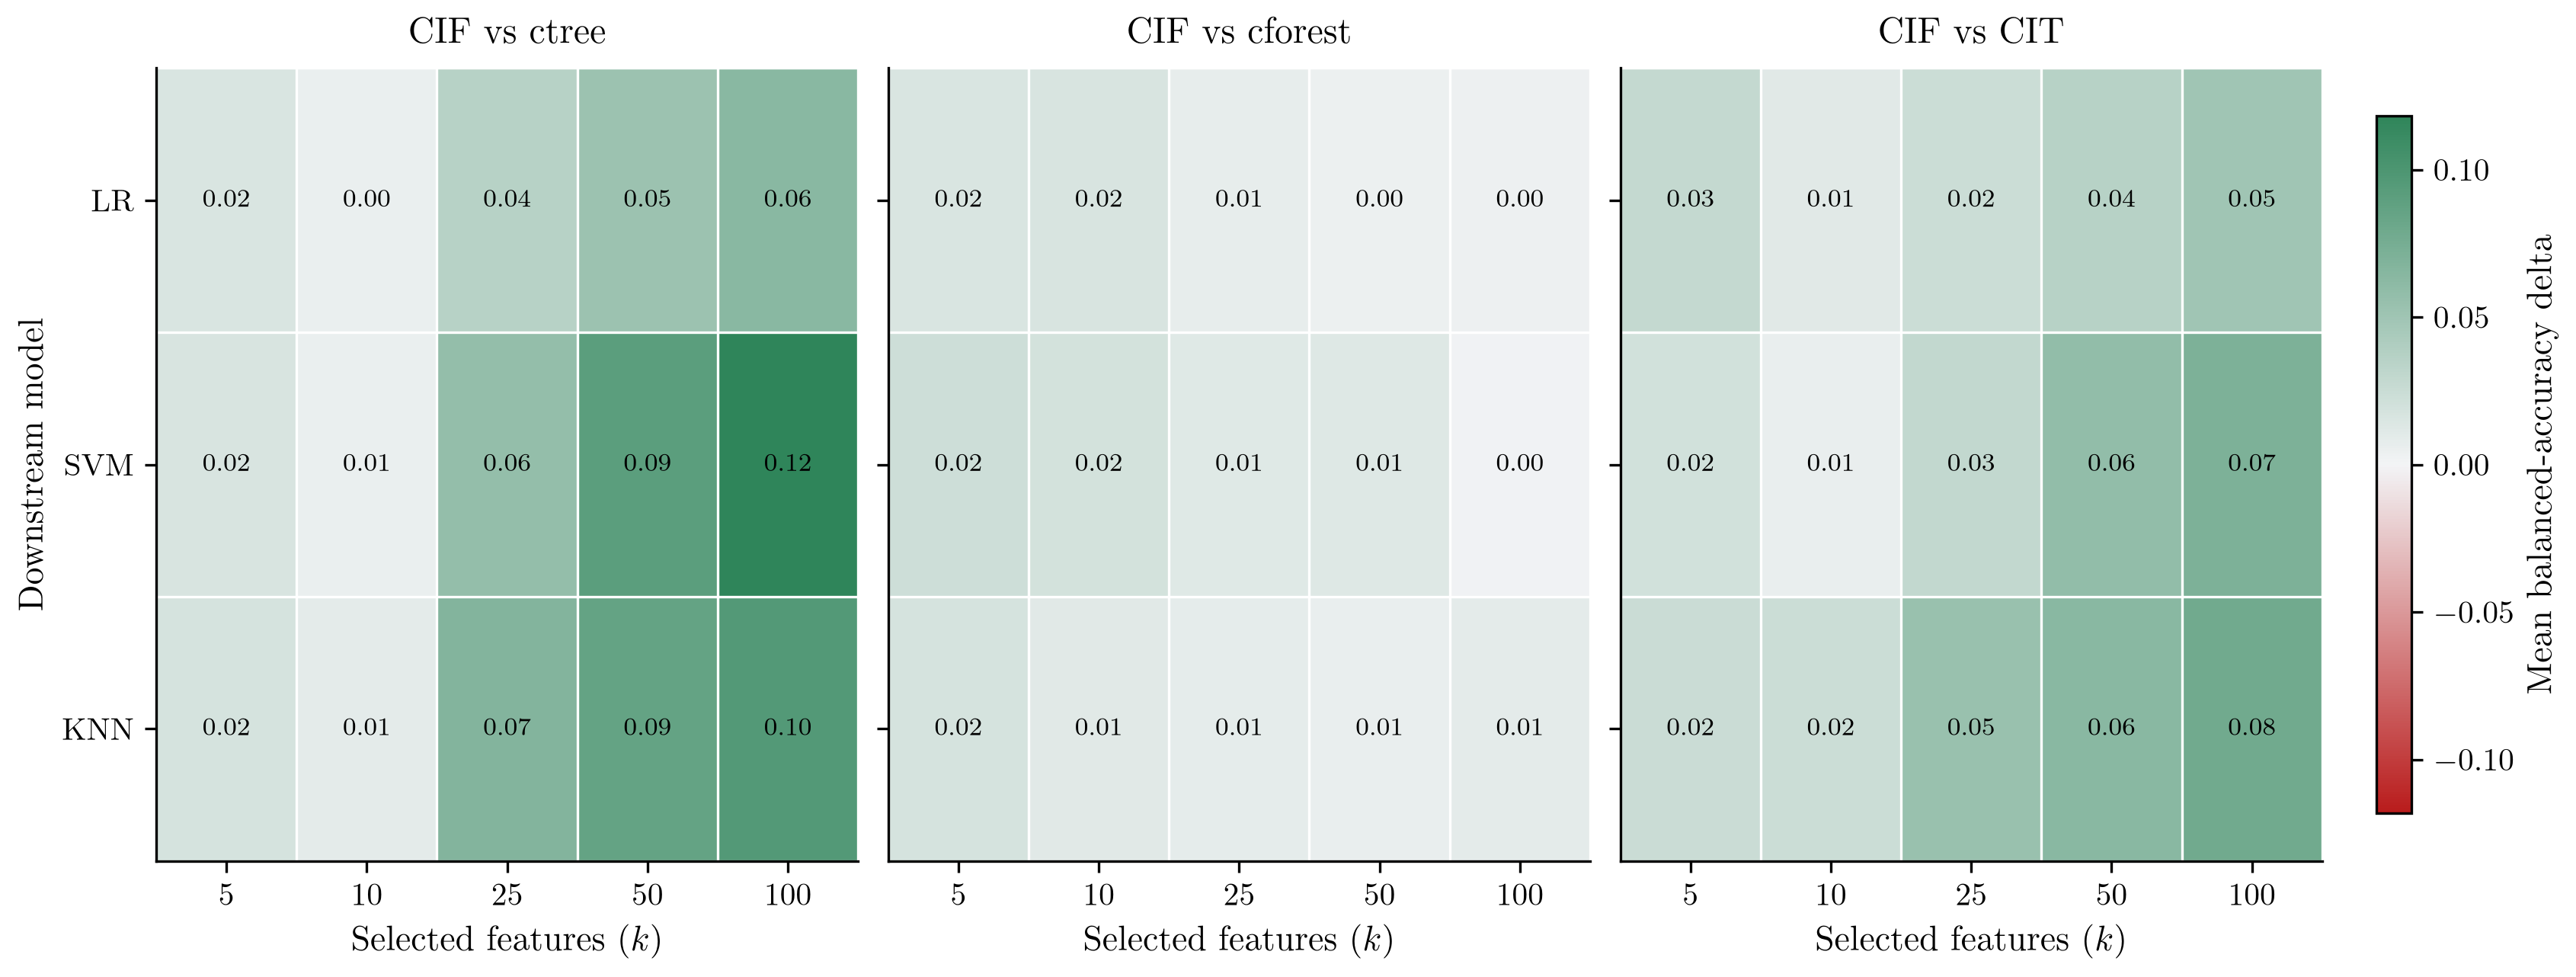
\includegraphics[width=0.88\linewidth]{figures/benchmark_pairwise_sensitivity.png}
  \caption{Classification CIF margins against ctree, cforest, and CIT by
  downstream learner and value of $k$. Each plotted value is the
  mean balanced-accuracy difference, CIF minus comparator, for one
  downstream learner and one value of $k$; positive values favor CIF. Dataset
  counts by $k$ are 21, 20, 14, 14, and 13 for ctree, 22, 21, 15, 15, and 14
  for cforest, and 23, 22, 16, 16, and 15 for CIT. Values are means over datasets; the bootstrap intervals for the pooled differences are in \cref{tab:conditional-inference-comparisons}.}
  \label{fig:benchmark-pairwise-sensitivity}
\end{figure}

\begin{figure}[!htbp]
  \centering
  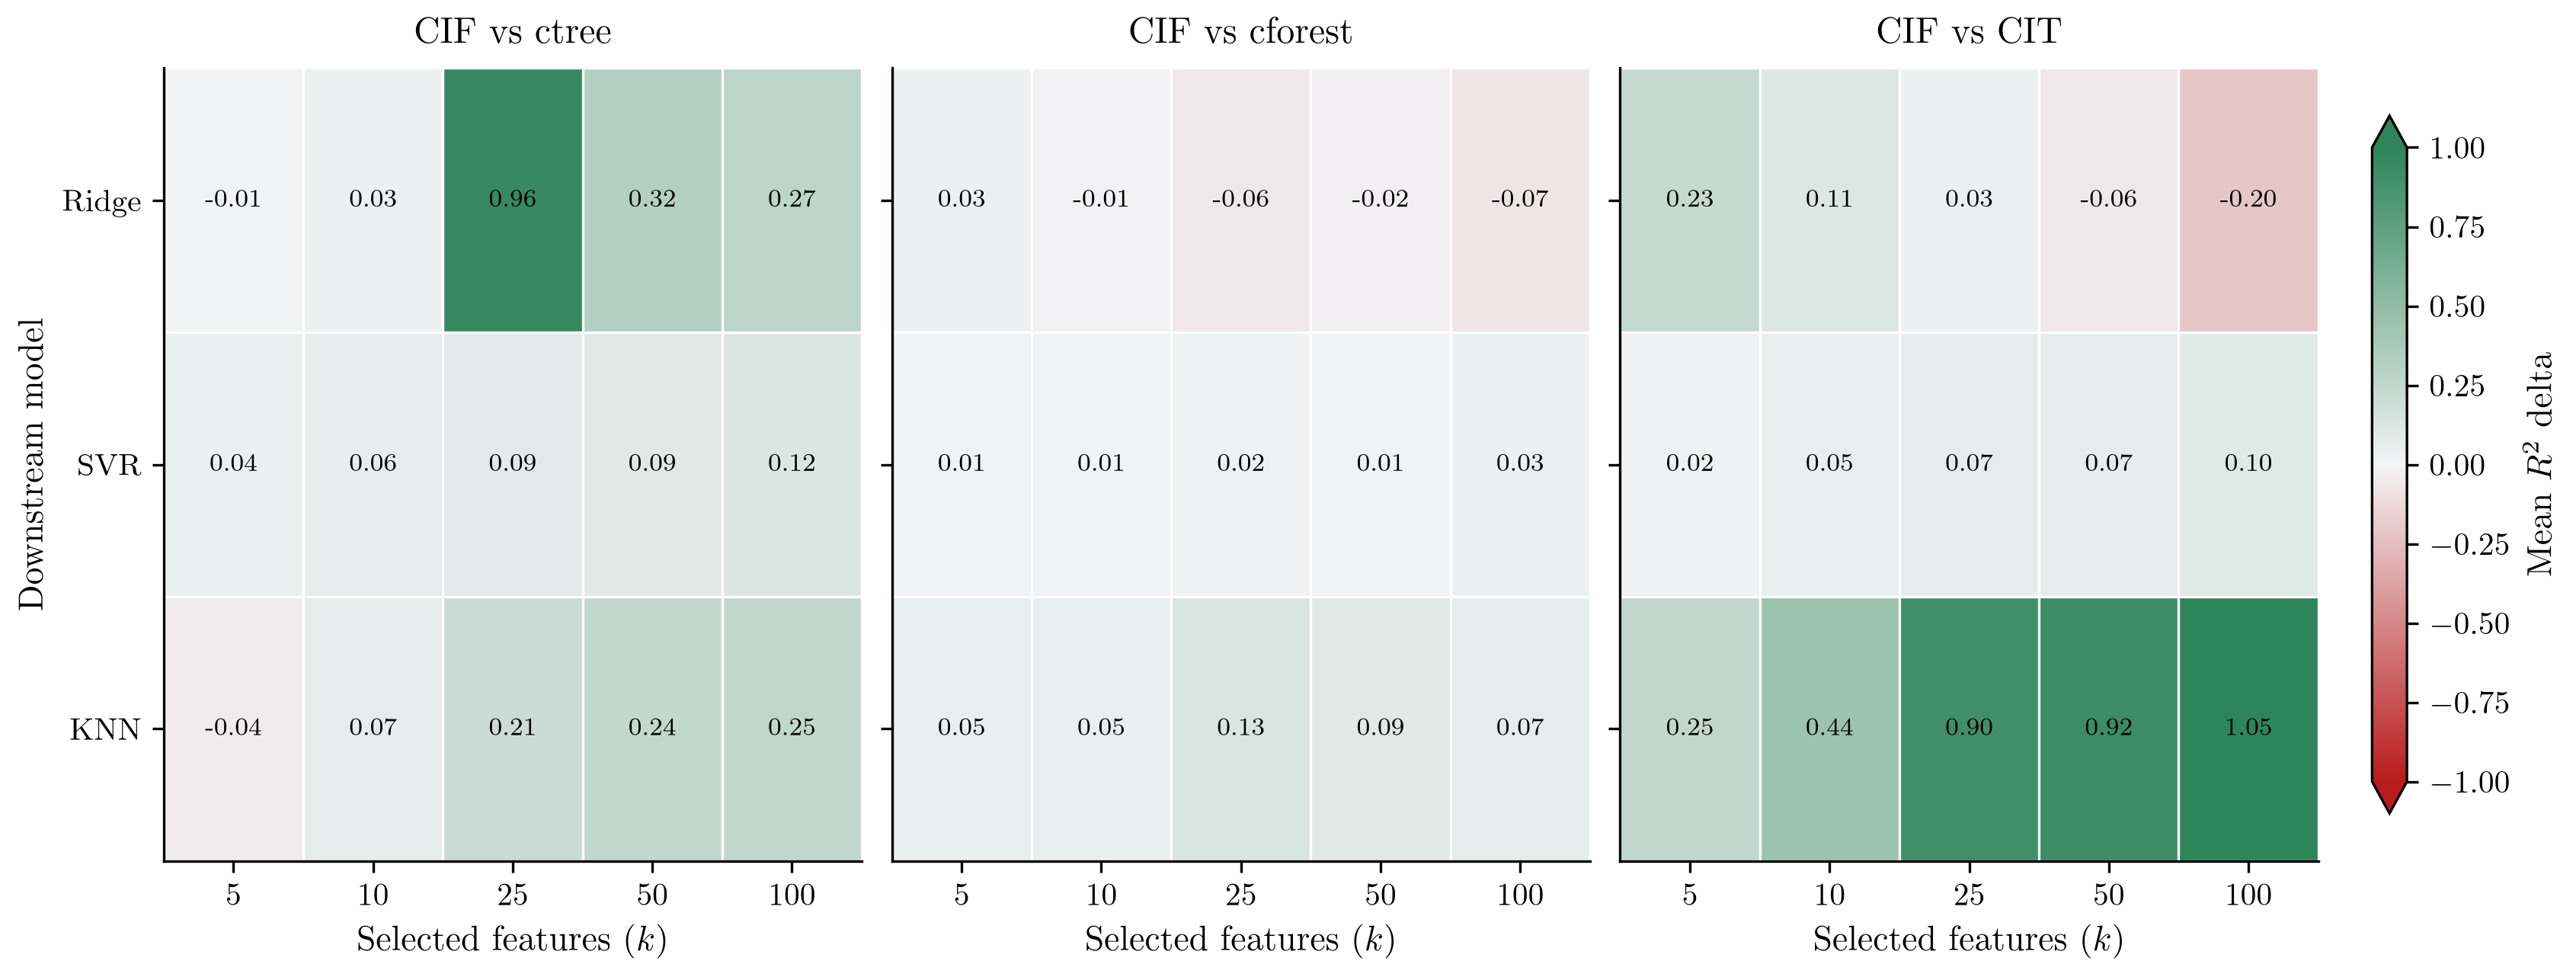
\includegraphics[width=0.88\linewidth]{figures/regression_benchmark_pairwise_sensitivity.png}
  \caption{Regression CIF margins against ctree, cforest, and CIT by
  downstream learner and value of $k$. Each plotted value is the mean
  $R^2$ difference, CIF minus comparator, for one downstream
  learner and one value of $k$; positive values favor CIF. Dataset counts by
  $k$ are 8, 8, 7, 7, and 6 for each comparison. Large positive plotted values
  can reflect negative mean $R^2$ for the comparator. Numeric labels show the
  unclipped values; the color scale is clipped at $\pm1$ for readability. Values are means over datasets; the bootstrap intervals for the pooled differences are in \cref{tab:conditional-inference-comparisons}.}
  \label{fig:regression-benchmark-pairwise-sensitivity}
\end{figure}

For the seed checks, each method is ranked separately within each fixed seed.
Keeping only datasets with results for every method, downstream learner,
standard top-$k$ value, and seed leaves 13 classification datasets and 6
regression datasets complete across all five seeds. These tables summarize seed
variation by rank without intervals or tests. In these tables, a seed column is
the method's ordinal position after sorting that seed's averaged dataset-level
ranks, while mean rank is the averaged dataset-level rank value itself. Rows
follow the main benchmark order. In classification CIF is 5th to 7th in every
seed (\cref{tab:classification-seed-sensitivity}), and in regression its
position ranges from 4th to 8th (\cref{tab:regression-seed-sensitivity}).

\begin{table}[!htbp]
  \centering
  \footnotesize
  \setlength{\tabcolsep}{4pt}
  \renewcommand{\arraystretch}{1.04}
  \begin{tabular}{@{}l
    S[table-format=2.0]
    S[table-format=2.0]
    S[table-format=2.0]
    S[table-format=2.0]
    S[table-format=2.0]
    S[table-format=2.1]
    S[table-format=2.1]@{}}
    \toprule
    \tablehead{Method} & {Seed 1} & {Seed 2} & {Seed 3} & {Seed 4} & {Seed 5} & {Mean position} & {Mean rank} \\
    \midrule
    RF-RFE & 1 & 1 & 1 & 1 & 1 & 1.0 & 4.9 \\
    XGBoost & 2 & 4 & 2 & 3 & 3 & 2.8 & 5.8 \\
    CIF & 6 & 5 & 6 & 5 & 7 & 5.8 & 6.9 \\
    RF & 5 & 6 & 4 & 6 & 4 & 5.0 & 6.6 \\
    LightGBM & 3 & 2 & 3 & 2 & 2 & 2.4 & 5.6 \\
    Boruta & 7 & 7 & 8 & 7 & 8 & 7.4 & 7.6 \\
    CatBoost & 4 & 3 & 5 & 4 & 5 & 4.2 & 6.4 \\
    ExtraTrees & 8 & 8 & 7 & 8 & 6 & 7.4 & 7.5 \\
    cforest & 9 & 9 & 9 & 9 & 9 & 9.0 & 8.3 \\
    DT & 10 & 10 & 11 & 10 & 10 & 10.2 & 9.6 \\
    RDC filter & 11 & 11 & 12 & 13 & 12 & 11.8 & 10.4 \\
    PI & 16 & 16 & 16 & 16 & 16 & 16.0 & 14.2 \\
    MC filter & 13 & 14 & 14 & 14 & 15 & 14.0 & 11.1 \\
    RT & 15 & 15 & 15 & 15 & 14 & 14.8 & 11.6 \\
    ctree & 14 & 12 & 10 & 12 & 11 & 11.8 & 10.4 \\
    CIT & 12 & 13 & 13 & 11 & 13 & 12.4 & 10.5 \\
    CPI & 17 & 17 & 17 & 17 & 17 & 17.0 & 15.7 \\
    \bottomrule
  \end{tabular}
  \caption{Classification seed sensitivity on the 13 datasets complete across
  all five seeds. Each seed column is the method's ordinal position after
  sorting methods by their averaged dataset-level ranks for that seed. Mean
  position averages those five ordinal positions; mean rank reports the averaged
  dataset-level rank value itself. Lower values are better. The spread across seed columns is the reported sensitivity.}
  \label{tab:classification-seed-sensitivity}
\end{table}

\begin{table}[!htbp]
  \centering
  \footnotesize
  \setlength{\tabcolsep}{4pt}
  \renewcommand{\arraystretch}{1.04}
  \begin{tabular}{@{}l
    S[table-format=2.0]
    S[table-format=2.0]
    S[table-format=2.0]
    S[table-format=2.0]
    S[table-format=2.0]
    S[table-format=2.1]
    S[table-format=2.1]@{}}
    \toprule
    \tablehead{Method} & {Seed 1} & {Seed 2} & {Seed 3} & {Seed 4} & {Seed 5} & {Mean position} & {Mean rank} \\
    \midrule
    ExtraTrees & 3 & 2 & 3 & 3 & 3 & 2.8 & 7.4 \\
    CIF & 6 & 5 & 8 & 8 & 4 & 6.2 & 8.6 \\
    CatBoost & 2 & 7 & 4 & 1 & 1 & 3.0 & 7.4 \\
    RF-RFE & 1 & 1 & 1.5 & 4 & 2 & 1.9 & 7.2 \\
    RF & 5 & 3 & 5 & 7 & 7 & 5.4 & 8.5 \\
    RT & 4 & 4 & 1.5 & 5 & 6 & 4.1 & 8.2 \\
    cforest & 15 & 13 & 13 & 12 & 11 & 12.8 & 10.2 \\
    DT & 14 & 6 & 7 & 2 & 5 & 6.8 & 8.6 \\
    Boruta & 9 & 10 & 10 & 11 & 8 & 9.6 & 9.3 \\
    PC filter & 16 & 16 & 15 & 14 & 16 & 15.4 & 11.3 \\
    LightGBM & 8 & 9 & 9 & 10 & 10 & 9.2 & 9.3 \\
    XGBoost & 7 & 8 & 11 & 6 & 12 & 8.8 & 9.2 \\
    RDC filter & 10 & 14 & 14 & 13 & 14 & 13.0 & 10.4 \\
    CIT & 12 & 12 & 17 & 17 & 9 & 13.4 & 10.7 \\
    ctree & 13 & 15 & 12 & 15 & 13 & 13.6 & 10.6 \\
    PI & 11 & 11 & 6 & 9 & 15 & 10.4 & 9.7 \\
    DC filter & 17 & 17 & 16 & 16 & 17 & 16.6 & 11.9 \\
    CPI & 18 & 18 & 18 & 18 & 18 & 18.0 & 12.8 \\
    \bottomrule
  \end{tabular}
  \caption{Regression seed sensitivity on the 6 datasets complete across all
  five seeds. Each seed column is the method's ordinal position after sorting
  methods by their averaged dataset-level ranks for that seed; fractional
  positions indicate ties. Mean position
  averages those five ordinal positions; mean rank reports the averaged
  dataset-level rank value itself. Lower values are better. The spread across seed columns is the reported sensitivity.}
  \label{tab:regression-seed-sensitivity}
\end{table}

\FloatBarrier
% Supplement Section S2: wide data and synthetic recovery (Figure 3, Figure 4, full synthetic recovery table).

\FloatBarrier
\section{Threshold test comparison tables}
\label{app:stageB-tables}

The threshold test comparison of \cref{sec:experiments-stageB} caps the
histogram candidates at the number of distinct values in the node and runs
five seeds unless stated otherwise. The null calibration uses 2,000 replicates
per cell and seed. The power study makes the response depend on the first
predictor through a step at zero, with class-probability shift
$\delta\in\{0.05,0.10,0.20\}$ or mean shift $\delta\in\{0.2,0.4,0.8\}$ and 500
replicates per cell and seed, and records the rates of any split and of a split
on the planted predictor and the error of the chosen threshold. The
Stage-B-only study runs nominal Stage~B levels from 0.02 to 0.50, with 500 null
replicates per cell, level, and seed over three seeds and 200 replicates of the
planted step, and interpolates power within each cell to a common realized
size of 0.05, or to the largest size both rules reach; its per-threshold test
without the threshold correction runs at nominal 0.05 with 500 null replicates
per cell. Two reruns check the matched comparison, one with a fourth seed of
1,500 null and 1,000 alternative replicates and one with the step moved from the
median to the 85th percentile of the predictor. The scaling study times one
tree on ten Gaussian predictors with a planted linear signal in three of them,
at $n\in\{1{,}000,4{,}000,16{,}000\}$, as the median of three fits with a
1,200-second cap. The real-data study fits one tree on the six Stage~B real
datasets at 256 bins with five-fold cross-validation, recording held-out score,
tree depth, fitting time, and the Spearman agreement of the two rules' feature
importances. The head-to-head timing fits each 100-tree forest once, with the
MC selector, the minimum budget, the two corrections, scanning, muting, the
256-bin histogram, and depth at most 3, on the ten head-to-head datasets and a
synthetic grid of Gaussian predictors with a weak or strong planted signal,
from $n=500$ to $32{,}000$ and $p=20$ to $500$.

\Cref{tab:stageB-calibration} gives the null calibration of the threshold test
comparison in \cref{sec:results-stageB}, whose design is in
\cref{sec:experiments-stageB}, and supports its statement that both Stage~B
rules keep the false-split rate of the whole node decision below 0.05 in every
cell. The rates of 0.0355 to 0.049 without the threshold correction quoted
there come from the same design at 2,000 replicates per cell, where every split
must still pass the Stage~A test first.

\Cref{tab:stageB-only-full} extends \cref{tab:stageB-only} with the sizes under
no stopping, which support the statement in its caption that they agree with
the sizes under adaptive stopping. Over both modes the per-threshold size is
0.000 to 0.027 and the max-type size 0.023 to 0.044. Over the 108 cell and
effect combinations the size-matched difference in power ranges from $-0.054$
to $+0.034$ and has no trend in the bin setting. In five cells the
per-threshold rule does not reach size 0.05 even at nominal 0.50, and the match
is at the largest size both rules reach. The two reruns give size-matched
differences of $-0.006$ ($-0.008$ to $-0.003$) at the fourth seed and $-0.004$
($-0.008$ to $0.000$) with the step at the 85th percentile, with standard
errors of about 0.017 and 0.038 on each difference. The standard errors come
from a parametric bootstrap of the whole matching procedure and put the
smallest detectable difference at about 0.03 for the fourth seed and 0.08 for
the step at the 85th percentile; the sizes in both reruns stay in the ranges
above. The max-type rule also places the threshold less precisely: on each
rule's own detections its threshold sits a median 0.19 standard deviations
from the planted cut against 0.15, and 87\% of its detections fall on the
planted predictor against 90\%.

\Cref{tab:stageB-power} gives the split rates at a common nominal level, whose
gap between the rules \cref{sec:results-stageB} attributes to the lower
realized size of the per-threshold rule. \Cref{tab:stageB-scaling} gives the
single-tree fitting times behind its cost comparison. Adaptive stopping
shortens the per-threshold test by 1.2 to 1.6, 2.2 to 3.2, and 3.8 to 7.8
times at 16, 64, and 256 bins, which narrows the max-type advantage to 1.0 to
1.3, 1.4 to 2.1, and 2.2 to 7.7. Held at 999 permutations per candidate
instead, the per-threshold rule never splits at 64 or 256 bins, because
$\alpha/K$ falls below the resolution $1/(B+1)$. Fitted depths barely differ,
5.0 to 10.7 levels for the max-type rule against 4.0 to 10.0. On the ten
head-to-head datasets the max-type forest reduces madelon from 21 to 2.6
seconds, gamma from 44 to 21, and isolet from 18 to 9.1, and changes the other
seven by at most 1.6 seconds.

\Cref{tab:stageB-real} gives the held-out scores, fitting times, and depths
behind the real-data comparison. The max-type rule scores higher by 0.016 and
0.026 balanced accuracy on vowel, 0.049 and 0.026 $R^2$ on facebook, 0.060 and
0.033 on imports-85, and 0.008 and 0.005 on residential, and lower by 0.018 and
0.020 on page-blocks and by 0.006 on spam with adaptive stopping. It fits 1.2
to 2.4 times faster with adaptive stopping and 1.0 to 8.3 times faster with no
stopping on the four datasets whose nodes admit many candidates, and 16\% and
10\% slower on residential. Fitted depths
agree within about one level (4.8 to 12.4 levels for the max-type rule against
5.4 to 11.4).

\begin{table}[!htbp]
  \centering
  \footnotesize
  \setlength{\tabcolsep}{5pt}
  \begin{tabular}{@{}lrrcccc@{}}
    \toprule
     & & & \multicolumn{2}{c}{Per-threshold} & \multicolumn{2}{c}{Max-type} \\
    \cmidrule(lr){4-5}\cmidrule(l){6-7}
    \tablehead{Task} & $n$ & Bins & Adaptive & No stopping & Adaptive & No stopping \\
    \midrule
    Classification & 100 & 16 & 0.018 & 0.018 & 0.034 & 0.035 \\
     & 100 & 64 & 0.013 & 0.013 & 0.035 & 0.037 \\
     & 100 & 256 & 0.009 & 0.010 & 0.036 & 0.038 \\
     & 200 & 16 & 0.020 & 0.020 & 0.033 & 0.034 \\
     & 200 & 64 & 0.014 & 0.015 & 0.033 & 0.034 \\
     & 200 & 256 & 0.009 & 0.009 & 0.033 & 0.035 \\
     & 500 & 16 & 0.020 & 0.020 & 0.030 & 0.031 \\
     & 500 & 64 & 0.014 & 0.014 & 0.032 & 0.033 \\
     & 500 & 256 & 0.007 & 0.007 & 0.032 & 0.034 \\
    Regression & 100 & 16 & 0.027 & 0.027 & 0.032 & 0.033 \\
     & 100 & 64 & 0.017 & 0.019 & 0.034 & 0.035 \\
     & 100 & 256 & 0.014 & 0.015 & 0.034 & 0.035 \\
     & 200 & 16 & 0.028 & 0.029 & 0.032 & 0.035 \\
     & 200 & 64 & 0.023 & 0.024 & 0.035 & 0.037 \\
     & 200 & 256 & 0.012 & 0.013 & 0.036 & 0.038 \\
     & 500 & 16 & 0.026 & 0.026 & 0.029 & 0.030 \\
     & 500 & 64 & 0.020 & 0.020 & 0.029 & 0.031 \\
     & 500 & 256 & 0.011 & 0.011 & 0.029 & 0.032 \\
    \bottomrule
  \end{tabular}
  \caption{False-split rate of a depth-one tree under the global null at level
  0.05, by Stage~B rule and stopping mode, over 10,000 replicates per cell
  (five seeds of 2,000). The tree has five independent Gaussian predictors and
  an independent response, and the rate covers Stage~A followed by Stage~B.
  Bins is the histogram setting. Every 95\% Clopper-Pearson interval lies below
  0.05, with largest upper limit 0.042.}
  \label{tab:stageB-calibration}
\end{table}

\begin{table}[!htbp]
  \centering
  \footnotesize
  \setlength{\tabcolsep}{4pt}
  \begin{tabular}{@{}lrrrrrrrrr@{}}
    \toprule
     & & & \multicolumn{4}{c}{Size at nominal 0.05} & & \multicolumn{2}{c}{Size-matched power} \\
     & & & \multicolumn{2}{c}{Per-threshold} & \multicolumn{2}{c}{Max-type} & Match & & \\
    \tablehead{Task} & $n$ & Bins & Adaptive & None & Adaptive & None & size & Per-threshold & Max-type \\
    \midrule
    Classification & 100 & 16 & 0.013 & 0.013 & 0.032 & 0.033 & 0.050 & 0.390 & 0.379 \\
     & 100 & 64 & 0.007 & 0.007 & 0.036 & 0.039 & 0.044 & 0.385 & 0.354 \\
     & 100 & 256 & 0.007 & 0.007 & 0.036 & 0.042 & 0.034 & 0.335 & 0.318 \\
     & 200 & 16 & 0.010 & 0.011 & 0.037 & 0.039 & 0.050 & 0.643 & 0.618 \\
     & 200 & 64 & 0.008 & 0.009 & 0.035 & 0.039 & 0.050 & 0.630 & 0.615 \\
     & 200 & 256 & 0.003 & 0.003 & 0.039 & 0.039 & 0.031 & 0.562 & 0.538 \\
     & 500 & 16 & 0.015 & 0.015 & 0.032 & 0.037 & 0.050 & 0.958 & 0.953 \\
     & 500 & 64 & 0.007 & 0.007 & 0.029 & 0.035 & 0.050 & 0.961 & 0.964 \\
     & 500 & 256 & 0.000 & 0.001 & 0.023 & 0.032 & 0.034 & 0.958 & 0.952 \\
    Regression & 100 & 16 & 0.019 & 0.019 & 0.023 & 0.031 & 0.050 & 0.292 & 0.281 \\
     & 100 & 64 & 0.013 & 0.013 & 0.029 & 0.035 & 0.050 & 0.305 & 0.285 \\
     & 100 & 256 & 0.011 & 0.010 & 0.031 & 0.037 & 0.050 & 0.317 & 0.299 \\
     & 200 & 16 & 0.027 & 0.026 & 0.033 & 0.038 & 0.050 & 0.591 & 0.581 \\
     & 200 & 64 & 0.017 & 0.017 & 0.033 & 0.043 & 0.050 & 0.619 & 0.598 \\
     & 200 & 256 & 0.008 & 0.009 & 0.041 & 0.044 & 0.050 & 0.632 & 0.579 \\
     & 500 & 16 & 0.026 & 0.026 & 0.031 & 0.032 & 0.050 & 0.947 & 0.942 \\
     & 500 & 64 & 0.015 & 0.016 & 0.029 & 0.033 & 0.050 & 0.966 & 0.952 \\
     & 500 & 256 & 0.005 & 0.006 & 0.026 & 0.034 & 0.046 & 0.963 & 0.951 \\
    \bottomrule
  \end{tabular}
  \caption{Stage-B-only study: the threshold test in isolation, with one
  Gaussian predictor fixed without the response and the Stage~A test disabled.
  Size is the false-split rate of a depth-one tree at nominal level 0.05 over
  1,500 null replicates per cell (three seeds of 500) under adaptive stopping
  and no stopping (None); every 95\% Clopper-Pearson upper limit is below
  0.056. Size-matched power, shown for adaptive stopping at the middle effect
  ($\delta = 0.10$ in classification, $0.4$ in regression), is interpolated
  against realized size over the nominal grid from 0.02 to 0.50 (600 replicates
  per cell and level) to the match size: 0.05, or the largest realized size
  both rules reach where the per-threshold rule does not reach 0.05.}
  \label{tab:stageB-only-full}
\end{table}

\begin{table}[!htbp]
  \centering
  \footnotesize
  \setlength{\tabcolsep}{4pt}
  \begin{tabular}{@{}lrrrrrrrr@{}}
    \toprule
     & & & \multicolumn{3}{c}{Per-threshold} & \multicolumn{3}{c}{Max-type} \\
    \tablehead{Task} & Effect & $n$ & 16 & 64 & 256 & 16 & 64 & 256 \\
    \midrule
    Classification & 0.05 & 100 & 0.036 & 0.025 & 0.020 & 0.058 & 0.060 & 0.061 \\
     & 0.05 & 200 & 0.058 & 0.047 & 0.033 & 0.084 & 0.088 & 0.088 \\
     & 0.05 & 500 & 0.159 & 0.148 & 0.107 & 0.192 & 0.193 & 0.193 \\
     & 0.10 & 100 & 0.126 & 0.104 & 0.092 & 0.170 & 0.170 & 0.172 \\
     & 0.10 & 200 & 0.315 & 0.296 & 0.247 & 0.362 & 0.360 & 0.364 \\
     & 0.10 & 500 & 0.820 & 0.813 & 0.786 & 0.828 & 0.830 & 0.832 \\
     & 0.20 & 100 & 0.698 & 0.676 & 0.658 & 0.727 & 0.729 & 0.730 \\
     & 0.20 & 200 & 0.971 & 0.972 & 0.968 & 0.972 & 0.972 & 0.972 \\
     & 0.20 & 500 & 1.000 & 1.000 & 1.000 & 1.000 & 1.000 & 1.000 \\
    Regression & 0.2 & 100 & 0.040 & 0.031 & 0.026 & 0.050 & 0.051 & 0.054 \\
     & 0.2 & 200 & 0.079 & 0.066 & 0.045 & 0.086 & 0.091 & 0.090 \\
     & 0.2 & 500 & 0.178 & 0.167 & 0.118 & 0.184 & 0.189 & 0.189 \\
     & 0.4 & 100 & 0.126 & 0.104 & 0.092 & 0.137 & 0.143 & 0.144 \\
     & 0.4 & 200 & 0.326 & 0.297 & 0.246 & 0.332 & 0.338 & 0.340 \\
     & 0.4 & 500 & 0.809 & 0.797 & 0.774 & 0.809 & 0.814 & 0.811 \\
     & 0.8 & 100 & 0.634 & 0.617 & 0.602 & 0.643 & 0.647 & 0.651 \\
     & 0.8 & 200 & 0.962 & 0.962 & 0.955 & 0.963 & 0.964 & 0.963 \\
     & 0.8 & 500 & 1.000 & 1.000 & 1.000 & 1.000 & 1.000 & 1.000 \\
    \bottomrule
  \end{tabular}
  \caption{Split rate at nominal level 0.05 of a depth-one tree with adaptive
  stopping when the response depends on one of five Gaussian predictors through
  a step at zero, by Stage~B construction and bin setting (columns 16, 64, 256),
  over 2,500 replicates per cell (five seeds of 500). The two rules have
  different realized sizes at this level (\cref{tab:stageB-calibration}), so
  the columns compare split rates rather than power; \cref{tab:stageB-only}
  compares power at equal size. Effect is the class-probability
  shift $\pm\delta$ around one half in classification and the mean shift in
  standard-deviation units in regression. No stopping agrees within
  0.014 in every cell.}
  \label{tab:stageB-power}
\end{table}

\begin{table}[!htbp]
  \centering
  \footnotesize
  \setlength{\tabcolsep}{4pt}
  \begin{tabular}{@{}lrrrrrrrr@{}}
    \toprule
     & & & \multicolumn{2}{c}{Adaptive} & \multicolumn{3}{c}{No stopping} & \\
    \tablehead{Task} & $n$ & Bins & Per-threshold & Max-type & Per-threshold & Fixed & Max-type & Fixed depth \\
    \midrule
    Classification & 1,000 & 16 & 0.04 & 0.04 & 0.05 & 0.04 & 0.06 & 5 \\
     & 1,000 & 64 & 0.07 & 0.04 & 0.20 & 0.06 & 0.11 & 0 \\
     & 1,000 & 256 & 0.45 & 0.09 & 3.52 & 0.24 & 0.28 & 0 \\
     & 4,000 & 16 & 0.12 & 0.11 & 0.19 & 0.14 & 0.22 & 6 \\
     & 4,000 & 64 & 0.31 & 0.15 & 0.99 & 0.22 & 0.47 & 0 \\
     & 4,000 & 256 & 1.83 & 0.31 & 14.2 & 0.86 & 1.35 & 0 \\
     & 16,000 & 16 & 0.47 & 0.37 & 0.75 & 0.55 & 0.93 & 8 \\
     & 16,000 & 64 & 1.11 & 0.59 & 3.57 & 0.89 & 2.10 & 0 \\
     & 16,000 & 256 & 9.36 & 1.22 & 59.0 & 3.46 & 6.28 & 0 \\
    Regression & 1,000 & 16 & 0.06 & 0.05 & 0.07 & 0.06 & 0.08 & 6 \\
     & 1,000 & 64 & 0.10 & 0.07 & 0.22 & 0.06 & 0.15 & 0 \\
     & 1,000 & 256 & 0.22 & 0.10 & 0.84 & 0.22 & 0.30 & 0 \\
     & 4,000 & 16 & 0.17 & 0.15 & 0.22 & 0.18 & 0.26 & 8 \\
     & 4,000 & 64 & 0.37 & 0.22 & 1.10 & 0.20 & 0.54 & 0 \\
     & 4,000 & 256 & 1.29 & 0.40 & 8.77 & 0.79 & 1.39 & 0 \\
     & 16,000 & 16 & 0.59 & 0.50 & 0.82 & 0.65 & 1.03 & 10 \\
     & 16,000 & 64 & 1.12 & 0.71 & 3.31 & 0.84 & 2.15 & 0 \\
     & 16,000 & 256 & 7.51 & 1.39 & 54.5 & 3.26 & 6.27 & 0 \\
    \bottomrule
  \end{tabular}
  \caption{Fitting time in seconds of one tree on ten Gaussian predictors with a
  planted linear signal, by Stage~B rule and stopping mode. All arms are timed in one run of five
  seeds; each entry is the median over seeds of the median of three timed fits,
  and each timed fit follows an untimed identical fit, so compilation is
  excluded. Bins is the histogram setting. Fixed is the
  per-threshold rule held at 999 permutations per candidate; it exists only with
  no stopping because the sequential path raises any budget to the floor
  $\lceil K/\alpha \rceil$, and Fixed depth is its fitted depth (0 where it never
  splits, because $\alpha/K < 1/1000$). No fit reached the 1,200-second cap.}
  \label{tab:stageB-scaling}
\end{table}

\begin{table}[!htbp]
  \centering
  \footnotesize
  \setlength{\tabcolsep}{4pt}
  \begin{tabular}{@{}lrrlrrrrrr@{}}
    \toprule
     & & & & \multicolumn{3}{c}{Adaptive} & \multicolumn{3}{c}{No stopping} \\
    \cmidrule(lr){5-7}\cmidrule(l){8-10}
    \tablehead{Dataset} & $n$ & $p$ & \tablehead{Rule} & Score & Seconds & Depth & Score & Seconds & Depth \\
    \midrule
    vowel & 990 & 10 & Per-threshold & 0.689 & 0.23 & 10.0 & 0.691 & 0.57 & 10.0 \\
     & & & Max-type & 0.705 & 0.15 & 11.2 & 0.717 & 0.40 & 11.4 \\
    \addlinespace
    spam & 4,601 & 57 & Per-threshold & 0.908 & 0.86 & 11.2 & 0.908 & 3.03 & 11.4 \\
     & & & Max-type & 0.902 & 0.71 & 12.4 & 0.908 & 3.01 & 11.4 \\
    \addlinespace
    page-blocks & 5,473 & 10 & Per-threshold & 0.768 & 0.69 & 10.0 & 0.768 & 5.85 & 10.0 \\
     & & & Max-type & 0.750 & 0.29 & 11.2 & 0.748 & 1.45 & 10.0 \\
    \addlinespace
    imports-85 & 205 & 76 & Per-threshold & 0.638 & 0.07 & 5.4 & 0.638 & 0.17 & 5.4 \\
     & & & Max-type & 0.698 & 0.07 & 4.8 & 0.671 & 0.18 & 5.2 \\
    \addlinespace
    residential & 372 & 107 & Per-threshold & 0.925 & 0.49 & 6.4 & 0.926 & 2.30 & 6.4 \\
     & & & Max-type & 0.933 & 0.57 & 7.2 & 0.931 & 2.53 & 6.6 \\
    \addlinespace
    facebook & 500 & 21 & Per-threshold & 0.754 & 0.33 & 9.0 & 0.754 & 2.09 & 9.0 \\
     & & & Max-type & 0.803 & 0.15 & 9.8 & 0.780 & 0.25 & 8.6 \\
    \bottomrule
  \end{tabular}
  \caption{Five-fold held-out score (balanced accuracy for vowel, spam, and
  page-blocks; $R^2$ for imports-85, residential, and facebook), fitting time in
  seconds, and fitted depth of one tree at the 256-bin histogram setting, by
  Stage~B rule and stopping mode. Each entry is the median over five seeds of
  the fold assignment. Each time is the second of two identical fits, so
  compilation is excluded.}
  \label{tab:stageB-real}
\end{table}

\FloatBarrier
\section{Weak-signal cardinality designs}
\label{sup:cardinality}

\Cref{tab:weak-signal-cardinality} gives the top-ten composition, support, and
downstream score of each ranking in the weak-signal designs behind the
cardinality comparison of \cref{sec:results-stageB}. The random forest ranked by
out-of-bag permutation importance keeps the preference of impurity importance
for high-cardinality noise, with a 500-level share above that of impurity
importance at the two weaker signals in both tasks.

\begin{table}[!htbp]
  \centering
  \footnotesize
  \setlength{\tabcolsep}{5pt}
  \begin{tabular}{@{}lrlrrrrr@{}}
    \toprule
     & & & \multicolumn{3}{c}{Share of the top ten} & & \\
    \tablehead{Task} & Signal & Ranking & Informative & 500-level noise & Binary noise & Support & Score \\
    \midrule
    Classification & 0.05 & CIF & 0.31 & 0.26 & 0.31 & 37 & 0.52 \\
     & & CIF, max-type & 0.34 & 0.28 & 0.26 & 46 & 0.51 \\
     & & RF impurity & 0.42 & 0.38 & 0.00 & 70 & 0.52 \\
     & & RF permutation & 0.30 & 0.47 & 0.06 & 34 & 0.51 \\
     & 0.10 & CIF & 0.64 & 0.16 & 0.13 & 45 & 0.56 \\
     & & CIF, max-type & 0.66 & 0.20 & 0.06 & 53 & 0.55 \\
     & & RF impurity & 0.72 & 0.19 & 0.00 & 70 & 0.56 \\
     & & RF permutation & 0.49 & 0.36 & 0.02 & 36 & 0.56 \\
     & 0.20 & CIF & 0.95 & 0.04 & 0.01 & 59 & 0.68 \\
     & & CIF, max-type & 0.96 & 0.04 & 0.00 & 65 & 0.69 \\
     & & RF impurity & 0.99 & 0.01 & 0.00 & 70 & 0.69 \\
     & & RF permutation & 0.87 & 0.09 & 0.00 & 39 & 0.67 \\
    Regression & 0.05 & CIF & 0.26 & 0.24 & 0.40 & 17 & $-$0.11 \\
     & & CIF, max-type & 0.34 & 0.22 & 0.30 & 21 & $-$0.11 \\
     & & RF impurity & 0.43 & 0.38 & 0.00 & 70 & $-$0.11 \\
     & & RF permutation & 0.37 & 0.43 & 0.05 & 34 & $-$0.10 \\
     & 0.10 & CIF & 0.64 & 0.11 & 0.20 & 24 & $-$0.05 \\
     & & CIF, max-type & 0.65 & 0.13 & 0.15 & 28 & $-$0.04 \\
     & & RF impurity & 0.73 & 0.17 & 0.00 & 70 & $-$0.04 \\
     & & RF permutation & 0.57 & 0.27 & 0.01 & 37 & $-$0.06 \\
     & 0.20 & CIF & 0.95 & 0.03 & 0.02 & 36 & 0.28 \\
     & & CIF, max-type & 0.95 & 0.02 & 0.02 & 44 & 0.28 \\
     & & RF impurity & 0.99 & 0.01 & 0.00 & 70 & 0.29 \\
     & & RF permutation & 0.95 & 0.03 & 0.00 & 39 & 0.28 \\
    \bottomrule
  \end{tabular}
  \caption{Weak-signal designs with mixed-cardinality noise, $n = 1{,}000$.
  Ten informative standard normal features have marginal correlation with the
  response given by the Signal column; the noise is 25 columns of integer codes
  on 500 levels, 25 binary columns, and 10 Gaussian columns. Shares are the mean
  composition of each ranking's top ten over 25 fits (5 seeds by 5 folds;
  standard errors 0.01 to 0.03); the remainder is Gaussian noise. Support is
  the mean number of features with nonzero importance; Score is the held-out
  balanced accuracy or $R^2$ of the downstream learners on the top ten. A
  ranking indifferent to cardinality would give each of the 500-level and binary
  noise types 25/60 of the top-ten places not taken by informative features. CIF is
  the selected configuration with the MC selector in classification and the PC
  selector in regression; CIF, max-type adds the max-type Stage~B rule; RF
  permutation is the same random forest ranked by out-of-bag permutation
  importance.}
  \label{tab:weak-signal-cardinality}
\end{table}


\end{document}
